% Hasse diagram of the divisors of 60 (generated by figs_c1ch02.py).
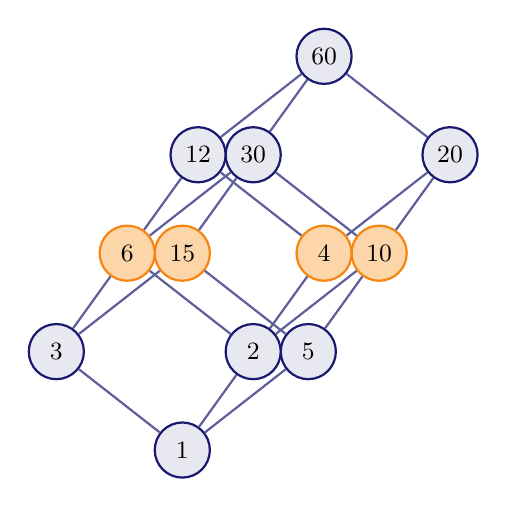
\begin{tikzpicture}[x=1cm,y=1cm,every node/.style={font=\small},d/.style={circle,draw=MidnightBlue,thick,fill=MidnightBlue!10,inner sep=1.5pt,minimum size=7mm}]
\node[d] (n1) at (0.00,0.00) {$1$};
\node[d] (n5) at (1.60,1.25) {$5$};
\node[d] (n3) at (-1.60,1.25) {$3$};
\node[d,fill=BurntOrange!30,draw=BurntOrange] (n15) at (0.00,2.50) {$15$};
\node[d] (n2) at (0.90,1.25) {$2$};
\node[d,fill=BurntOrange!30,draw=BurntOrange] (n10) at (2.50,2.50) {$10$};
\node[d,fill=BurntOrange!30,draw=BurntOrange] (n6) at (-0.70,2.50) {$6$};
\node[d] (n30) at (0.90,3.75) {$30$};
\node[d,fill=BurntOrange!30,draw=BurntOrange] (n4) at (1.80,2.50) {$4$};
\node[d] (n20) at (3.40,3.75) {$20$};
\node[d] (n12) at (0.20,3.75) {$12$};
\node[d] (n60) at (1.80,5.00) {$60$};
\draw[thick,MidnightBlue!70] (n1) -- (n2);
\draw[thick,MidnightBlue!70] (n1) -- (n3);
\draw[thick,MidnightBlue!70] (n1) -- (n5);
\draw[thick,MidnightBlue!70] (n5) -- (n10);
\draw[thick,MidnightBlue!70] (n5) -- (n15);
\draw[thick,MidnightBlue!70] (n3) -- (n6);
\draw[thick,MidnightBlue!70] (n3) -- (n15);
\draw[thick,MidnightBlue!70] (n15) -- (n30);
\draw[thick,MidnightBlue!70] (n2) -- (n4);
\draw[thick,MidnightBlue!70] (n2) -- (n6);
\draw[thick,MidnightBlue!70] (n2) -- (n10);
\draw[thick,MidnightBlue!70] (n10) -- (n20);
\draw[thick,MidnightBlue!70] (n10) -- (n30);
\draw[thick,MidnightBlue!70] (n6) -- (n12);
\draw[thick,MidnightBlue!70] (n6) -- (n30);
\draw[thick,MidnightBlue!70] (n30) -- (n60);
\draw[thick,MidnightBlue!70] (n4) -- (n12);
\draw[thick,MidnightBlue!70] (n4) -- (n20);
\draw[thick,MidnightBlue!70] (n20) -- (n60);
\draw[thick,MidnightBlue!70] (n12) -- (n60);
\end{tikzpicture}
